\subsubsection{Expansion Parallel Ports JP3}

The \systemName~includes two parallel ports that are connected to the
{\it JP3} expansion header on the \DEBoard~board. One of these parallel ports provides 13
bidirectional connections, and the other port provides three input-only connections. 
Each of the parallel ports includes the four 32-bit registers that were described previously for 
Figure~\ref{fig:parallel_port}. The base address of the 13-bit bidirectional port connected to 
{\it JP3} is {\sf 0xFF200080} and the base address of the input-only port is {\sf 0xFF200090}.
Figure \ref{fig:expansion_port_JP3} gives a diagram of the {\it JP3} expansion connector on 
the \DEBoard~board, and shows how both the bidirectional and input-only parallel ports are 
connected.  The figure shows that bits $D_0$ to $D_{12}$ of the bidirectional parallel port 
are assigned to pins 5 to 17 of the {\it JP3} connector. Bits {\it IN}$_0$ to 
{\it IN}$_2$ of the input-only parallel port are assigned to pins 2 to 4 of the connector.

\begin{figure}[h!]
   \begin{center}
       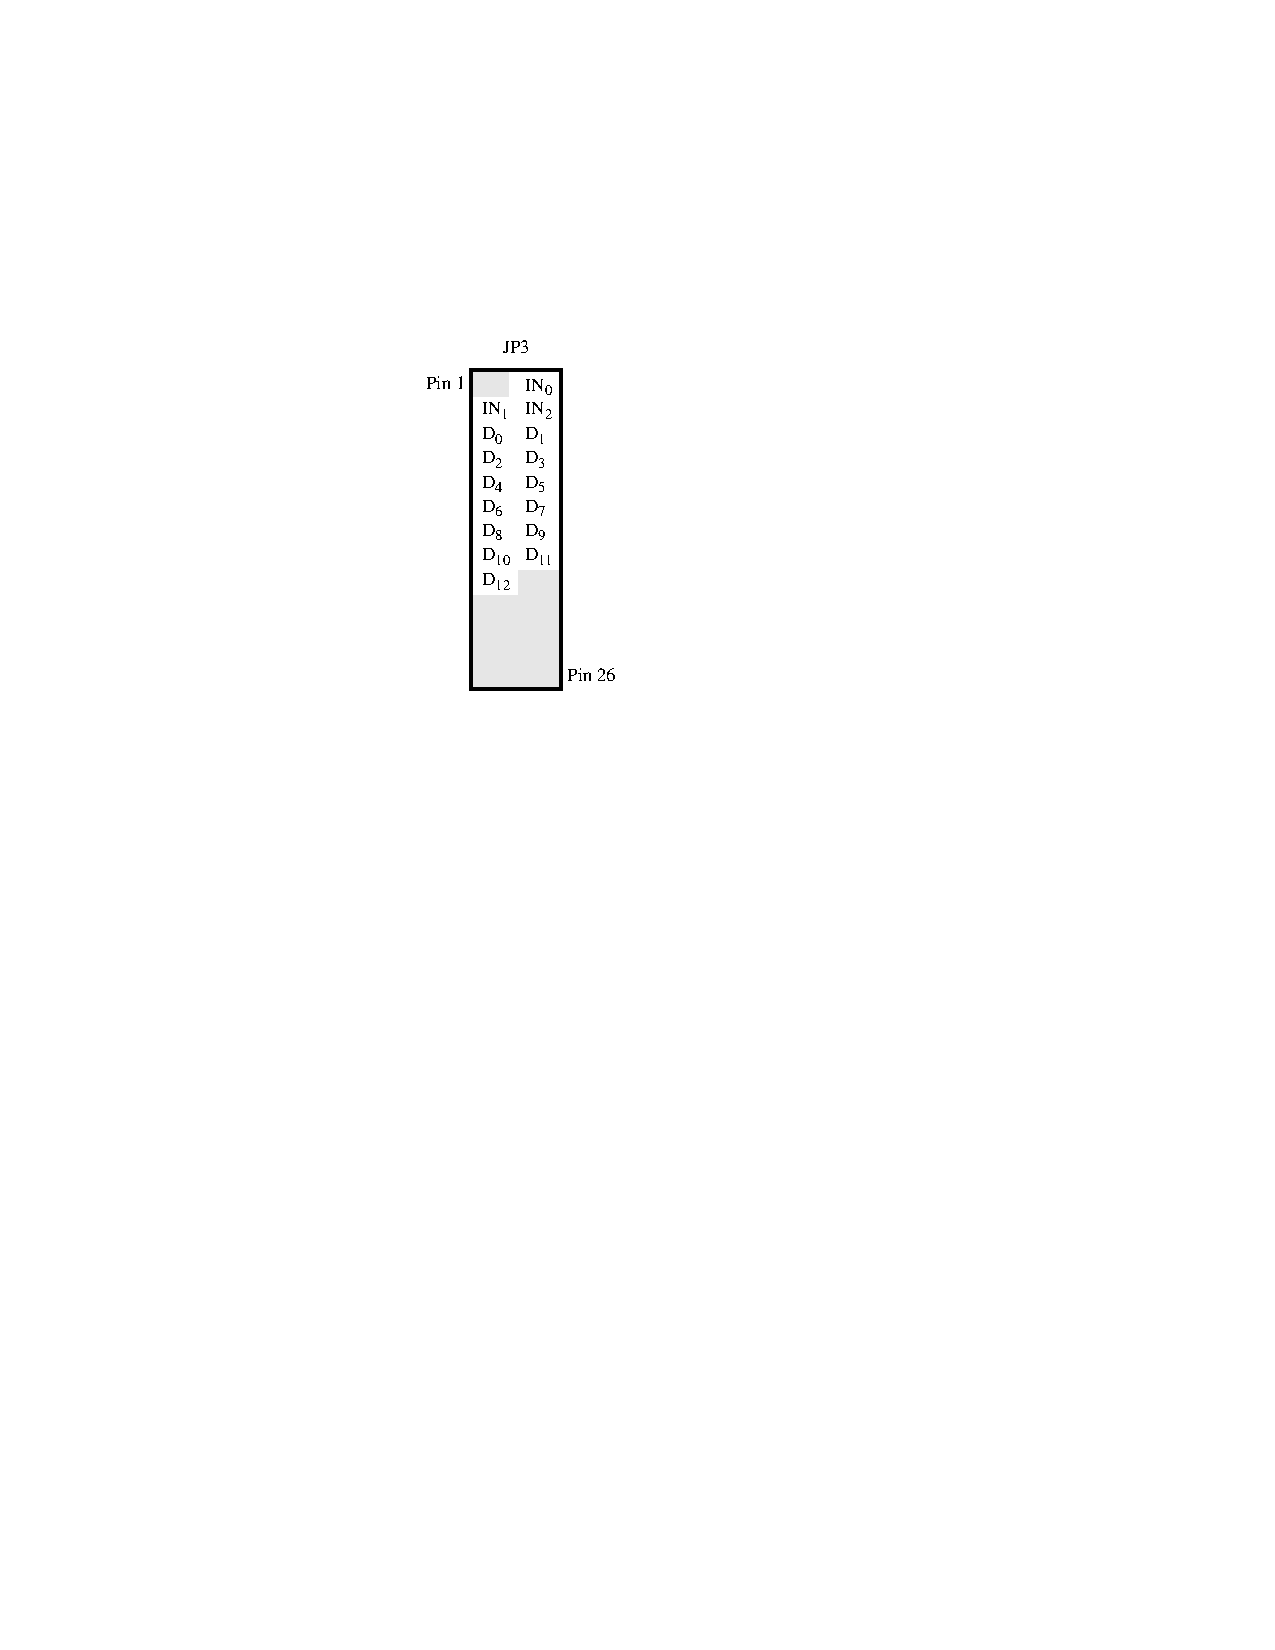
\includegraphics{\commonPath/../figs/FPGA_PP_Expansion_Port3.pdf}
   \end{center}
   \caption{Assignment of parallel port bits to pins on {\it JP3}.}
	\label{fig:expansion_port_JP3}
\end{figure}